% Manuscrito propio de trabajo, 12nov2026. No cambia geometría de la plantilla.
\documentclass[11pt]{article}
\usepackage[utf8]{inputenc}
\usepackage[T1]{fontenc}
\usepackage[spanish,es-nodecimaldot,es-noquoting]{babel}
\usepackage[margin=1in]{geometry}
\usepackage{lmodern,amsmath,amssymb,amsthm,booktabs,graphicx,array,xcolor}
\usepackage[round]{natbib}
\usepackage[colorlinks=true,allcolors=blue!50!black]{hyperref}
% Generated by code/verify.py. Do not edit numerical values.
\newcommand{\PEGapLow}{4.31}
\newcommand{\PEGapHigh}{10.43}
\newcommand{\PhiFormalFinal}{0.38}
\newcommand{\PhiHighFinal}{0.70}
\newcommand{\PEMOne}{51.71}
\newcommand{\PEMThree}{37.75}
\newcommand{\PENoCap}{0}
\newcommand{\PEMaxHours}{0.749}
\newcommand{\FixedZFinal}{1.037}
\newcommand{\WedgeMThreeRef}{37.36}
\newcommand{\WedgeMThreeConst}{20.96}
\newcommand{\WedgeMOneRef}{51.682}
\newcommand{\WedgeMThreeRefit}{37.364}
\newcommand{\WedgeVThreeRef}{4.399}
\newcommand{\WedgeVThreeRefit}{4.277}
\newcommand{\CountMATFinal}{17}
\newcommand{\CountGEFinal}{14}
\newcommand{\MotivationQOne}{94.0}
\newcommand{\MotivationQFive}{49.3}
\newcommand{\MeanAssetsFinal}{5.141}
\newcommand{\InterestRefFinal}{6.576}
\newcommand{\CapitalRefFinal}{5.165}
\newcommand{\FinalPERows}{%
0.38 & 33.997 & 0.40000 & 4.309 \\
0.45 & 19.495 & 0.40079 & 5.660 \\
0.50 & 14.424 & 0.40130 & 6.621 \\
0.60 & 9.191 & 0.40217 & 8.531 \\
0.70 & 6.671 & 0.40288 & 10.425 \\
}
\newcommand{\FinalWedgeRows}{%
Dos sectores & 51.682 & 37.364 & 4.399 & 1.463 \\
Prima constante & 51.682 & 37.368 & 4.399 & 1.463 \\
Barrera constante & 51.298 & 20.956 & 3.463 & 1.435 \\
Ambas constantes & 51.298 & 20.957 & 3.464 & 1.435 \\
Ambas, reajuste & 51.682 & 37.364 & 4.277 & 1.448 \\
}

\newtheorem{proposition}{Proposición}
\theoremstyle{definition}
\newtheorem{assumption}{Supuesto}
\newcommand{\Va}{V_a}
\newcommand{\Vaa}{V_{aa}}
\newcommand{\sI}{s_I}
\title{Ahorro, flexibilidad de horas e informalidad en el Perú\\[3pt]\large Un mecanismo laboral en un modelo macroeconómico de agentes heterogéneos}
\author{John Svante Barraza Ratachi\\ \small Universidad del Pacífico, AI and Economic Modeling, Track B\\
\small\url{https://github.com/johnbarraza/ai-project}}
\date{12 de noviembre de 2026. Manuscrito de trabajo para discusión}
\setlength{\emergencystretch}{2em}
\begin{document}
\maketitle
\begin{abstract}
Estudio cuándo la riqueza modifica el reparto de horas formales e informales a productividad fija. En un bloque laboral interior con desutilidad isoelástica separable, la elasticidad del cociente de horas respecto al valor marginal de los activos es la diferencia entre las elasticidades sectoriales. Si ese valor marginal disminuye con los activos, la fracción informal cae con la riqueza exactamente cuando la elasticidad informal es mayor. Con elasticidad común, el canal directo se cancela. Un ejercicio parcial reproduce el mecanismo y contrastes de equilibrio general muestran dependencia de la barrera formal. No se identifican efectos causales ni se prueba concavidad global de la HJB. Lean comprueba localmente la derivada de las políticas explícitas y sus signos; el flujo oficial sobre un paper publicado en commit sigue pendiente.
\end{abstract}

\section{Introducción}
El marco es una economía de equilibrio general con hogares heterogéneos, producción formal e informal y una distribución de activos. La pregunta individual importa para macro porque sus políticas se agregan mediante esa distribución, determinan oferta de trabajo y ahorro y deben ser compatibles con los precios de los mercados. La proposición estudia una pieza de ese circuito; los contrastes numéricos de equilibrio general muestran cómo la especificación se transmite también a precios y capital.

La informalidad puede asociarse tanto con la productividad de la persona como con los recursos que tiene disponibles. Esa asociación no dice por sí sola qué decisión cambiaría si dos hogares con igual productividad dispusieran de activos diferentes. La pregunta de este trabajo es más acotada: ¿cuándo influye la riqueza en el reparto de horas entre trabajo formal e informal, manteniendo la productividad laboral individual fija? La decisión considerada es una cantidad de horas en cada actividad. Ambos trabajos pueden coexistir; no se modela aquí la llegada de una oferta ni una elección discreta de sector.

La motivación descriptiva proviene de los agregados de ENAHO 2023 conservados en el proyecto. La tasa de empleo informal de personas ocupadas es \MotivationQOne\% en el quintil de menor gasto per cápita y \MotivationQFive\% en el de mayor gasto. Estos números fueron recuperados del archivo público de agregados y no se volvieron a estimar desde microdatos en esta revisión. Además, el gasto no es patrimonio y una tasa de personas no es una fracción de horas. El patrón sirve para formular la pregunta, pero no se usará como una meta directamente comparable con la brecha de horas por activos del modelo.

La respuesta es condicional. En el bloque de trabajo del hogar, ambas actividades reciben la misma valoración marginal de una unidad adicional de activos, \(\Va\). Si las dos desutilidades tienen la misma elasticidad, ese término aparece con el mismo exponente en ambas horas y desaparece al tomar su cociente. La riqueza puede modificar el trabajo total sin modificar directamente su composición a un mismo estado de productividad. Si las elasticidades difieren, el cociente hereda una potencia de \(\Va\). El signo por activos depende entonces de la diferencia de elasticidades y de la derivada de \(\Va\) respecto a la riqueza.

El resultado aporta un diagnóstico del mecanismo dentro del modelo de dos sectores. No se presenta como una demostración de prioridad frente a toda la literatura de oferta laboral. Permite identificar qué supuesto impide un canal directo de composición y qué condición lo recupera. También ayuda a distinguir ese canal del gradiente por productividad generado por la barrera formal y por el rendimiento de la productividad en el sector informal. Una relación agregada entre activos e informalidad puede existir incluso con elasticidad común si la distribución de productividad difiere entre grupos de riqueza.

El trabajo separa tres tareas. La primera es la demostración analítica de la proposición local. La segunda es una reproducción del ejercicio parcial de octubre, con precios, distribución y valor marginal fijos. La tercera utiliza los contrastes de cuñas de noviembre, en los que se resolvieron de nuevo precios y distribución en equilibrio general. Esa separación evita interpretar una sensibilidad parcial como un nuevo equilibrio y evita llamar identificación empírica al reajuste de dos momentos internos.

\section{Antecedentes y alcance}
El punto de partida es el ahorro bajo riesgo idiosincrático de \citet{Aiyagari1994}. La extensión relevante para este proyecto conserva activos y productividad heterogéneos, pero incorpora dos firmas, dos bienes y horas elegidas en ambas actividades. \citet{Achdou2022} desarrolla la formulación continua mediante una HJB para valor y políticas y una ecuación de Kolmogorov para la distribución. Su sección 2.1 presenta el entorno básico y su sección 7 discute extensiones. Esa referencia justifica el marco y el método; no identifica las elasticidades laborales de este proyecto.

El antecedente cercano para Perú es el Documento de Trabajo 2024-005 del BCRP, \citet{Galindo2024}. Su objeto es la relación entre informalidad y distribución de riqueza en un modelo de agentes heterogéneos. El documento se cita como trabajo de investigación del banco central; no se afirma aquí una publicación posterior arbitrada. En el manuscrito local revisado, el estado formal o informal es exógeno y el hogar elige consumo y ahorro. Aquí se estudia el reparto simultáneo de horas. Endogeneizar ese reparto intensivo no equivale a endogeneizar transiciones entre empleos excluyentes.

La revisión previa de supuestos también consideró \citet{Kaplan2018}. El tratamiento de una prima crediticia como costo de intermediación resulta útil para la contabilidad. No ofrece respaldo automático para imponer a la barrera laboral y a la prima de deuda una misma función decreciente de productividad. La coincidencia de letras entre artículos tampoco establece equivalencia económica. Por ello, los perfiles de cuñas se mantienen como elecciones del proyecto que requieren contraste.

La revisión de literatura es focalizada y su registro conserva límites de acceso y de lectura. No se declara exhaustiva la búsqueda de trabajos que citan a los antecedentes. Tampoco se atribuye a esas referencias una estimación de la desigualdad entre elasticidades formal e informal. Esa desigualdad es una sensibilidad ilustrativa del bloque de horas. El resultado teórico no depende de que tal orden se haya estimado para Perú, pero su aplicación cuantitativa sí necesita evidencia que lo discipline.

\section{Modelo y supuestos}
\subsection{Estados, información y decisiones}
El estado individual es \((a,z)\), donde \(a\) son activos y \(z>0\) es productividad laboral. Los activos evolucionan mediante el ahorro; la productividad sigue un proceso exógeno conocido por el hogar. En tiempo continuo el hogar elige consumos \(c_F,c_I\) y horas \(\ell_F,\ell_I\). Con una canasta CES \(C(c_F,c_I)\), sus preferencias son
\begin{equation}\label{eq:preferences}
\mathbb E_0\int_0^\infty e^{-\rho t}
\left[\ln C(c_F,c_I)-
\sum_{s\in\{F,I\}}\frac{\psi_s\ell_s^{1+1/\phi_s}}{1+1/\phi_s}\right]dt.
\end{equation}
La canasta distingue los dos bienes. El argumento de composición laboral usa la separabilidad del bloque de horas y su vínculo con la restricción de recursos; no requiere estimar aquí un nuevo parámetro de sustitución de consumo.

El precio formal se normaliza a uno y \(p_I\) es el precio relativo del bien informal. La ley de movimiento de activos es
\begin{equation}\label{eq:budget}
\dot a=R_F(z)\ell_F+R_I(z)\ell_I+ra-\chi(z)(-a)_+
+T-c_F-p_Ic_I,
\end{equation}
con \(a\geq\underline a\), \(\ell_s\geq0\) y
\(\ell_F+\ell_I\leq\bar H\). El hogar observa su estado actual y conoce la ley del riesgo, pero no su realización futura. Toma precios, remuneraciones efectivas y transferencias como dados al resolver su problema individual.

Los retornos por hora que recibe son
\begin{equation}\label{eq:returns}
R_F(z)=(1-\tau)w_Fz-\kappa(z),\qquad
R_I(z)=\widetilde w_Iz^{\nu_I}.
\end{equation}
La barrera se paga por hora formal, \(\kappa(z)\ell_F\). La prima se paga sobre deuda, \(\chi(z)(-a)_+\). Son objetos distintos: la primera no es un costo fijo de aceptación de empleo y la segunda no resuelve un problema endógeno de default.

\subsection{Producción, distribución y mercados}
La firma formal produce \(Y_F=A_FK_F^\alpha L_F^{1-\alpha}\) y elige capital y trabajo para maximizar \(Y_F-w_FL_F-(r+\delta)K_F\). La firma informal produce \(Y_I=A_IK_I^{\alpha_I}L_I^{\beta_I}\) y maximiza \(p_IY_I-w_IL_I-(r+\delta)K_I\). Se mantiene \(0<\alpha<1\), \(\alpha_I,\beta_I>0\) y \(\alpha_I+\beta_I<1\). Las FOC igualan productos marginales valorados a costos de factores. Los beneficios formales son cero y los informales son
\[
\Pi_I=(1-\alpha_I-\beta_I)p_IY_I,\qquad
\widetilde w_I=w_I+\Pi_I/L_I.
\]
El reparto de beneficios por trabajo efectivo es una convención del modelo. El retorno informal del hogar no debe confundirse con el salario que paga la firma.

Si \(\mu\) es la distribución de hogares, los agregados relevantes son
\[
S=\int a\,d\mu,\quad
L_F=\int z\ell_F\,d\mu,\quad
L_I=\int z^{\nu_I}\ell_I\,d\mu,\quad
C_s=\int c_s\,d\mu .
\]
Los mercados de activos y del bien informal exigen \(S=K_F+K_I\) y \(C_I=Y_I\). El gobierno devuelve la recaudación formal mediante \(T=\tau w_FL_F\). El cierre de recursos formales incluye ambos pagos de cuñas:
\begin{equation}\label{eq:formal_resources}
Y_F=C_F+\delta(K_F+K_I)+\mathcal K+\mathcal D,\quad
\mathcal K=\int\kappa(z)\ell_F\,d\mu,\quad
\mathcal D=\int\chi(z)(-a)_+\,d\mu .
\end{equation}
La ecuación de Kolmogorov determina la distribución estacionaria compatible con las políticas. En GE los precios y esa distribución vuelven a resolverse. La proposición siguiente mantiene la remuneración del problema individual fija.

\subsection{Condiciones del resultado local}
Escribo \(v(a,z)\) para el valor del hogar y \(\Va(a,z)=\partial_av(a,z)\). Cuando la solución es regular, el bloque laboral de la HJB es
\begin{equation}\label{eq:hoursblock}
\max_{\ell_F,\ell_I}
\left\{\Va(R_F\ell_F+R_I\ell_I)-
\sum_s\frac{\psi_s\ell_s^{1+1/\phi_s}}{1+1/\phi_s}\right\}.
\end{equation}
La derivación no constituye una prueba de regularidad de la HJB. Se explicitan las condiciones bajo las que puede usarse.

\begin{assumption}[Comparación individual]\label{ass:fixed}
Se fija \(z\) y se considera un entorno abierto de un punto \(a_0>\underline a\). Los retornos \(R_F,R_I>0\), los precios y las remuneraciones efectivas se mantienen fijos y no dependen directamente de los activos en esa comparación.
\end{assumption}
\begin{assumption}[Preferencias laborales]\label{ass:parameters}
Para \(s\in\{F,I\}\), \(\psi_s>0\) y \(\phi_s>0\). El costo de horas es el de \eqref{eq:preferences}, separable entre actividades.
\end{assumption}
\begin{assumption}[Rama interior regular]\label{ass:regular}
La función \(a\mapsto\Va(a,z)\) es positiva y diferenciable en \(a_0\). Las horas de la rama considerada satisfacen las FOC de \eqref{eq:hoursblock}, son positivas y su suma es estrictamente menor que \(\bar H\).
\end{assumption}
\begin{assumption}[Concavidad local para la interpretación]\label{ass:concavity}
Cuando se interpreta el signo por riqueza se mantiene \(\Vaa(a_0,z)<0\).
\end{assumption}

Los tres primeros supuestos permiten derivar la identidad. El cuarto solo se usa para ordenar sus signos. Su cumplimiento en una grilla no implica una demostración global. Si el tope de tiempo se activa, aparece un multiplicador común y la fórmula interior deja de ser la política correspondiente. Si se evalúa el límite de endeudamiento, se requieren derivadas unilaterales y un enunciado adaptado; ese caso no queda cubierto por el entorno abierto utilizado aquí.

\section{Resultado y prueba}
Defina la fracción de horas informales como
\(\sI=\ell_I/(\ell_F+\ell_I)\). Esta definición cuenta horas y no clasifica ex ante a una persona como informal. Bajo los retornos positivos y la rama interior, \(0<\sI<1\).

\begin{proposition}[Composición condicional de horas]\label{prop:composition}
Bajo los supuestos \ref{ass:fixed}--\ref{ass:regular}, la política interior satisface
\begin{equation}\label{eq:main}
\frac{\partial\sI(a_0,z)}{\partial a}
=\sI(a_0,z)\bigl(1-\sI(a_0,z)\bigr)
(\phi_I-\phi_F)\frac{\Vaa(a_0,z)}{\Va(a_0,z)} .
\end{equation}
Si además se cumple el supuesto \ref{ass:concavity}, la derivada es negativa cuando \(\phi_I>\phi_F\), cero cuando \(\phi_I=\phi_F\) y positiva cuando \(\phi_I<\phi_F\).
\end{proposition}

\begin{proof}
Derivar \eqref{eq:hoursblock} respecto a una hora positiva de la actividad \(s\), con el tiempo holgado, da
\[
\Va R_s-\psi_s\ell_s^{1/\phi_s}=0.
\]
La derivada del costo divide y multiplica por el mismo exponente \(1+1/\phi_s\); por eso no queda ese factor en la FOC. La segunda derivada de la función objetivo respecto a \(\ell_s>0\) es
\(-(\psi_s/\phi_s)\ell_s^{1/\phi_s-1}<0\). La rama interior tiene, por tanto, las políticas explícitas
\begin{equation}\label{eq:explicit}
\ell_s=\left(\frac{\Va R_s}{\psi_s}\right)^{\phi_s}.
\end{equation}
Todos los argumentos de las potencias son positivos. La composición considerada es la obtenida de estas políticas.

Sea \(q=\ell_I/\ell_F>0\). Al dividir \eqref{eq:explicit} se obtiene
\[
q=\frac{(R_I/\psi_I)^{\phi_I}}{(R_F/\psi_F)^{\phi_F}}
\Va^{\phi_I-\phi_F}.
\]
El coeficiente de la derecha no depende de \(a\), por el supuesto \ref{ass:fixed}. Tomar logaritmos y diferenciar da
\[
\frac{\partial\ln q}{\partial a}
=(\phi_I-\phi_F)\frac{\Vaa}{\Va},
\qquad
\frac{\partial q}{\partial a}
=q(\phi_I-\phi_F)\frac{\Vaa}{\Va}.
\]
La división por \(\Va\) es válida porque es positiva. Como
\(\sI=q/(1+q)\), la regla del cociente implica
\[
\frac{\partial\sI}{\partial a}
=\frac{\partial_aq}{(1+q)^2}
=\frac{q}{(1+q)^2}(\phi_I-\phi_F)\frac{\Vaa}{\Va}.
\]
Finalmente, \(q/(1+q)^2=\sI(1-\sI)\), lo que prueba \eqref{eq:main}. El factor \(\sI(1-\sI)/\Va\) es positivo. Si \(\Vaa<0\), multiplicarlo por \(\phi_I-\phi_F\) produce los tres signos indicados. En la igualdad de elasticidades, la diferencia es exactamente cero y la identidad se anula.
\end{proof}

El resultado no afirma que riqueza e informalidad sean independientes en toda la distribución cuando las elasticidades coinciden. Afirma que la composición individual interior no responde directamente a los activos a un mismo \(z\). Las distribuciones de productividad por grupos de activos pueden ser distintas, y ello puede generar una brecha agregada positiva. Tampoco se compara aquí una economía con otra: un cambio de parámetros que modifica precios, políticas y distribución requiere resolver el equilibrio y agregar nuevamente.

La igualdad de elasticidades es, por tanto, una frontera útil de sensibilidad. Por encima de la diagonal \(\phi_I=\phi_F\), el signo local es negativo bajo concavidad; por debajo es positivo. El mapa no representa regiones de existencia de un equilibrio ni probabilidades estimadas. Resume la álgebra de una proposición condicional.

\begin{figure}[htbp]
\centering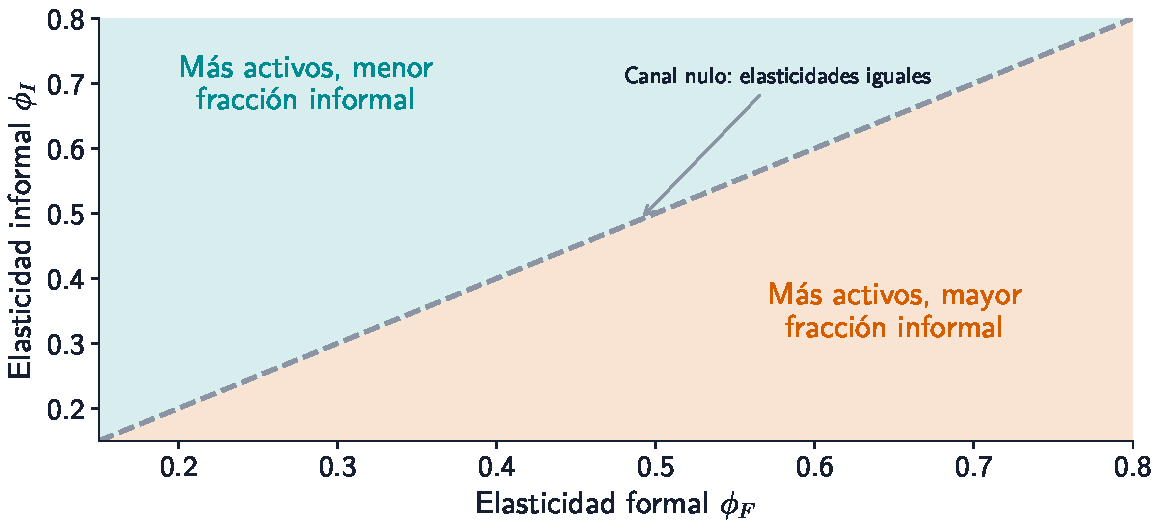
\includegraphics[width=.76\linewidth]{../code/figures/final/sign_map.pdf}
\caption{Signo de la derivada por activos bajo \(\Vaa<0\) y los demás supuestos de la proposición. Rango ilustrativo de elasticidades. Fuente: \texttt{code/verify.py}.}
\label{fig:sign}
\end{figure}

\section{Comprobaciones y ejercicios numéricos}
\subsection{Qué se reproduce}
El punto de entrada es \texttt{python code/verify.py}. El script comprueba las FOC por diferenciación simbólica y compara políticas explícitas con optimizaciones escalares independientes del objetivo. También verifica la derivada de la fracción y la regla de la cadena utilizada en \eqref{eq:main}. El procedimiento falla si una identidad o tolerancia declarada no se cumple. Estas comprobaciones detectan errores de implementación; una colección finita de casos no sustituye la demostración.

Se conservan dos fuentes numéricas. La primera es la exportación pública del cierre histórico, de \(200\times40\) nodos, desde la que se reconstruye el valor marginal compatible con las FOC. La segunda son exportaciones de diagnósticos de los contrastes D73 del 9 de noviembre. En esta revisión Python vuelve a producir el PE desde la primera fuente y relee los indicadores guardados de la segunda. No vuelve a resolver en MATLAB las HJB/KFE de D73. Los archivos de procedencia distinguen ambas operaciones.

Esta distinción también determina el significado de la palabra verificación. La identidad de composición tiene una prueba algebraica y una comprobación simbólica. El ejercicio parcial tiene una reproducción numérica. Las corridas D73 conservan una auditoría independiente realizada sobre sus MAT y sus diagnósticos exportados, pero no se les atribuye una nueva ejecución en esta sesión. Finalmente, la estabilidad frente a grilla y dominio es un problema separado del cierre de una corrida individual.

\subsection{Sensibilidad parcial de las elasticidades}
El experimento mantiene precios, \(V_a\) y distribución de la exportación histórica. Para cada elasticidad informal se reajustan \(\psi_I\) y el nivel de la barrera de modo que se recuperen los momentos internos M1 y M3 de esa misma referencia. M1 es la razón de horas informales agregadas a horas totales. M3 es la diferencia de fracciones formales entre extremos de productividad. No son, respectivamente, una tasa de personas ni una estimación directa por educación.

La figura \ref{fig:assets} muestra la fracción informal por activos en un mismo nodo de productividad. Con elasticidad común, la curva es plana. Con elasticidad informal mayor, desciende. El reajuste puede alterar niveles e intersecciones; la proposición fija el signo local, no exige que todas las curvas pasen por el mismo punto.

\begin{figure}[htbp]
\centering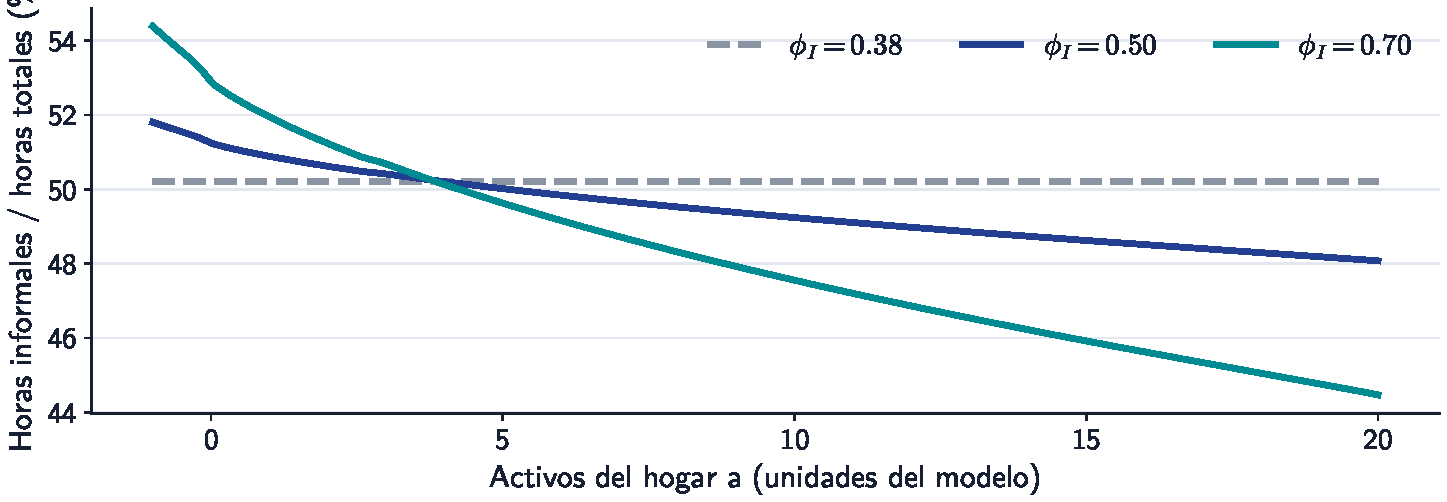
\includegraphics[width=.85\linewidth]{../code/figures/final/assets.pdf}
\caption{Fracción de horas informales por activos, con \(z=\FixedZFinal\) y \(\phi_F=\PhiFormalFinal\). PE con distribución, precios y \(V_a\) fijos; reajuste a M1/M3 internos. Fuente: \texttt{code/verify.py}.}
\label{fig:assets}
\end{figure}

\begin{table}[htbp]
\centering
\caption{Sensibilidad parcial con M1/M3 internos mantenidos}
\label{tab:pe}
\begin{tabular}{rrrr}\toprule
\(\phi_I\)&\(\psi_I\)&Nivel de barrera&V3 D17 (pp)\\\midrule
\FinalPERows\bottomrule
\end{tabular}
\par\smallskip\footnotesize V3 es la diferencia Q1--Q5 de fracciones de horas informales por activos. M1 = \PEMOne\%, M3 = \PEMThree\ pp. No es una recalibración a datos nuevos.
\end{table}

La brecha V3 aumenta de \PEGapLow\ a \PEGapHigh\ puntos en el rango considerado. La tabla utiliza la convención D17, que incorpora el nodo que cruza el corte de Q1. El código histórico también conserva la convención antigua de MATLAB, que produce cifras próximas, pero distintas. No se intercambian esas definiciones dentro de una comparación. La magnitud no se interpreta como reducción de una brecha empírica: los descriptivos de personas por gasto y el resultado de horas por activos no comparten denominador ni variable de clasificación.

\subsection{Cuñas en equilibrio general}
Los contrastes D73 utilizan el modelo simultáneo original con elasticidad común. Comparan la referencia con prima constante, barrera constante y ambas constantes. Los niveles constantes iniciales igualan pagos agregados evaluados con las políticas de referencia. Esa igualdad inicial no garantiza pagos iguales después de resolver el GE. En cada contraste se ajustan precios, políticas y distribución y se comprueban mercados, HJB, KFE y condiciones laborales.

El bloque amplio utiliza \(400\times40\) nodos y dominio de activos de \(-1\) a \(40\). La figura \ref{fig:wedges} y la tabla \ref{tab:ge} muestran que hacer constante la prima cambia poco los momentos mostrados. Hacer constante la barrera reduce M3 de \WedgeMThreeRef\ a \WedgeMThreeConst\ puntos, con los otros parámetros mantenidos. El gradiente por productividad depende, por tanto, de una forma que el modelo impone. Este es un diagnóstico de sensibilidad, no una estimación del costo de acceder al sector formal.

\begin{figure}[htbp]
\centering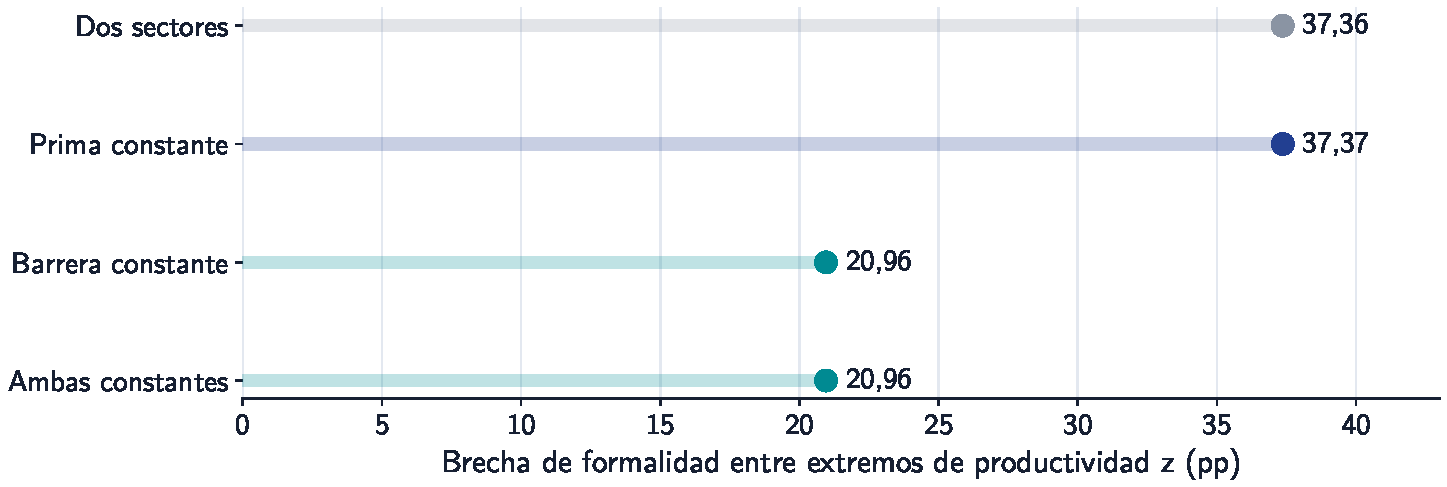
\includegraphics[width=.85\linewidth]{../code/figures/final/wedges.pdf}
\caption{M3 en contrastes GE de forma a otros parámetros fijos. Constantes iniciales igualan pagos de referencia. Los precios se resuelven de nuevo. Fuente: exportaciones D73 verificadas por \texttt{code/verify.py}.}
\label{fig:wedges}
\end{figure}

\begin{table}[htbp]
\centering
\caption{Cuñas y reajuste en GE, dominio amplio}
\label{tab:ge}
\begin{tabular}{lrrrr}\toprule
Caso&M1 (\%)&M3 (pp)&V3 (pp)&Gasto F/I\\\midrule
\FinalWedgeRows\bottomrule
\end{tabular}
\par\smallskip\footnotesize V3 usa quintiles de activos con reparto fraccional del nodo de corte. El gasto clasifica hogares por sector dominante en horas. No mezclar V3 con la convención D17.
\end{table}

Un contraste adicional reajusta \(\psi_I\) y el nivel constante de \(\kappa\) para recuperar M1/M3 del GE de referencia de la misma grilla. Ambas formas recuperan esas metas internas, pero producen V3 de \WedgeVThreeRef\ y \WedgeVThreeRefit\ puntos. La razón de gasto tampoco mejora frente a la meta registrada de 1,913; esa meta se conserva como dato del paquete, sin nueva revalidación de microdatos. Ajustar dos momentos puede disciplinar parámetros dentro de una familia sin identificar cuál forma funcional es la correcta entre familias.

\subsection{Transmisión a precios y capital}
La distribución estacionaria es el puente entre las políticas del hogar y los agregados. La exportación histórica permite reconstruir la distribución marginal de activos y sumar horas con sus ponderaciones. El ahorro agregado es $S=\MeanAssetsFinal$ en unidades de ese modelo, mientras que la participación informal de horas es \PEMOne\%. La razón de horas agregadas no equivale al promedio simple de las fracciones individuales: hogares que trabajan cantidades distintas tienen pesos distintos en el denominador.

En los GE D73 el capital debe ser consistente con los activos agregados. Se agregó a la reproducción la identidad entre el exceso de activos guardado y la diferencia de ahorro y demanda de capital. La figura \ref{fig:macro_ge} muestra los cambios de la tasa de interés y del capital respecto al GE de referencia de la misma grilla. La escala de interés está en puntos básicos y la de capital en cambio porcentual. No se trata de una trayectoria temporal. Estos resultados describen diferencias estacionarias entre especificaciones; no se interpretan como una intervención identificada ni como efectos de bienestar.

\begin{figure}[htbp]
\centering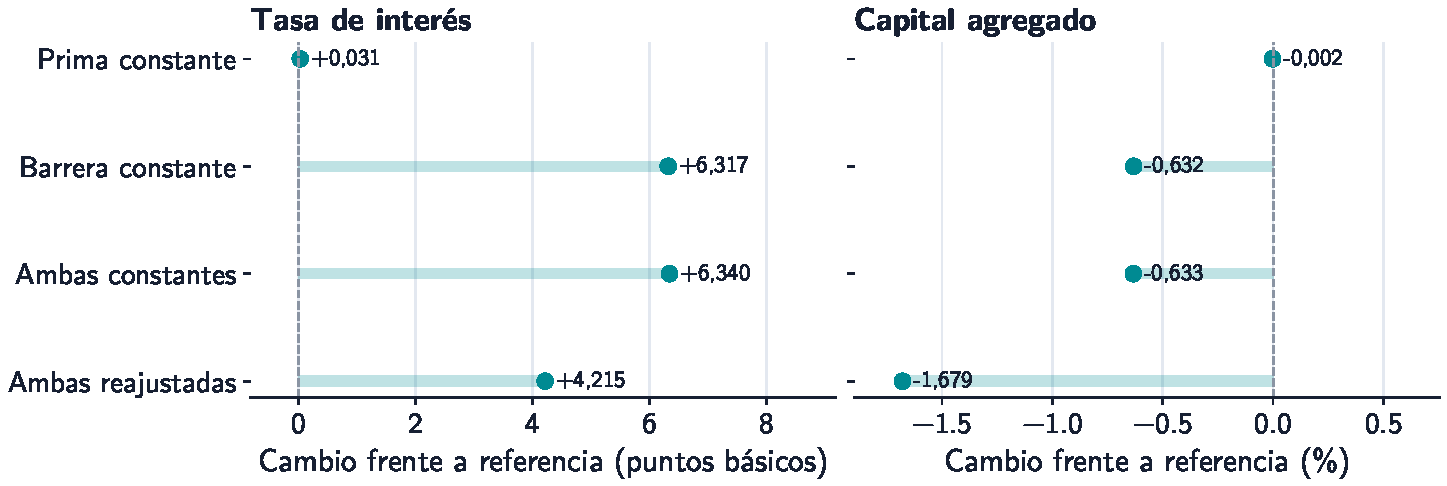
\includegraphics[width=.85\linewidth]{../code/figures/final/macro_ge.pdf}
\caption{Ajuste de precios y capital en los GE D73 amplios. Referencia: $r=\InterestRefFinal\%$ y $K=\CapitalRefFinal$ unidades del modelo. Fuente: exportaciones de las mismas corridas auditadas, reproducidas por \texttt{code/verify.py}.}
\label{fig:macro_ge}
\end{figure}

\subsection{Diagnósticos y límites de precisión}
El registro D73 conserva \CountMATFinal\ MAT auditados, de los cuales \CountGEFinal\ son GE. Los controles distinguen masa, generador, HJB, KFE, unicidad de clase cerrada, factibilidad, FOC y mercados. Un indicador agregado pequeño no basta si su fórmula omite un costo real. La revisión previa encontró un indicador histórico que excluía la prima de deuda; los contrastes nuevos verifican los dos pagos de \eqref{eq:formal_resources}. El fallo histórico no se borra ni se reutiliza como certificación de los nuevos resultados.

La ampliación del dominio reduce masa en la frontera superior, pero quedan dos pares finos comparables en el mismo dominio amplio y una revisión de resolución o truncamiento de \(z\). No se declara certificación global de precisión. Cambiar los extremos de productividad puede modificar el perfil normalizado de una cuña y no solo su resolución; por eso las anclas económicas deben mantenerse al hacer comparaciones de grilla. Tampoco se cambia silenciosamente el límite de endeudamiento para que converja un caso.

\section{Discusión y limitaciones}
La proposición identifica el papel de la igualdad de elasticidades y de la concavidad local. Su fuerza consiste en aislar ese canal; su límite consiste en las condiciones que requiere. Un hogar en una esquina sectorial, en el tope de tiempo o en un punto sin derivabilidad exige otro enunciado. Esos casos no pueden incorporarse mediante la misma fórmula solo porque el solver entregue un número. La extensión a un cambio de precios también añade términos que aquí se mantienen constantes.

El resultado agregado requiere integrar políticas con una distribución. Una brecha positiva entre quintiles de activos no contradice la cancelación a \(z\) fijo, porque la productividad puede estar distribuida de manera distinta entre quintiles. Del mismo modo, una brecha parcial mayor al variar una elasticidad no demuestra que un GE tenga el mismo cambio. Recalcular equilibrio es una tarea distinta y el manuscrito no afirma haberla completado para las elasticidades de sensibilidad.

La interpretación empírica sigue siendo una limitación sustantiva. Las referencias revisadas no estiman automáticamente \(\phi_I-\phi_F\), \(\nu_I\) o el perfil compartido de cuñas del proyecto. La medición por personas, horas, ingreso, gasto y patrimonio debe reconciliarse antes de juzgar ajuste. Para distinguir especificaciones después de un reajuste, hacen falta momentos externos que no se hayan utilizado para igualarlas. Comparar solo el tamaño de V3 favorecería una forma por el resultado deseado, sin identificar su mecanismo.

Lean comprueba la derivada y los signos de las políticas explícitas, con la condición de concavidad declarada. No prueba regularidad o concavidad de la HJB ni existencia del GE. Quedan pendientes el flujo oficial sobre un commit publicado, el manuscrito personal y la revisión semántica del autor.

\section{Conclusión}
A igual productividad y dentro de una rama laboral interior, la composición de horas responde al valor marginal de los activos mediante la diferencia de elasticidades sectoriales. Con valor marginal decreciente en riqueza, una elasticidad informal mayor produce una fracción informal decreciente; la igualdad de elasticidades cancela el canal directo. El ejercicio parcial reproduce esa lógica y los contrastes GE muestran dependencia del gradiente por productividad respecto a la barrera formal. La conclusión es condicional y no causal. Los pasos siguientes son disciplinar empíricamente los parámetros, construir indicadores comparables y cerrar los requisitos de formalización y manuscrito con su procedencia completa.
\label{body:end}
\clearpage
\bibliographystyle{plainnat}
\bibliography{references}
\appendix

\section{Correspondencia con Lean}\label{app:lean}
La fuente propia es \texttt{lean/LaborComposition.lean}. La comprobación local se ejecutó con Lean 4.30.0-rc2 y Mathlib fijado en el commit indicado por \texttt{lean/lakefile.toml}. La salida y el hash de fuente están en \texttt{lean/verification/local\_check.json}. Los únicos axiomas reportados son los estándar de Mathlib: \texttt{propext}, \texttt{Classical.choice} y \texttt{Quot.sound}; no aparece \texttt{sorryAx}.

\begin{center}\small
\begin{tabular}{p{2.6cm}p{7.3cm}p{4cm}}\toprule
Resultado&Declaraciones, prefijo \texttt{Barraza26LaborComposition}&Estado\\\midrule
Proposición \ref{prop:composition}, identidad&\texttt{composition\_hasDerivAt}&Probada para políticas explícitas, comprobación local\\
Proposición \ref{prop:composition}, signos&\texttt{composition\_sign}&Probados bajo \(\Vaa<0\), ya declarada en el paper\\\bottomrule
\end{tabular}
\end{center}

El código define \texttt{labor v R psi phi = (v*R/psi)\^{}phi} y \texttt{share} como la fracción de horas de \eqref{eq:explicit}. La función \texttt{V} representa \(a\mapsto\Va(a,z)\), mientras \texttt{d} representa su derivada. \texttt{HasDerivAt V d a} es una hipótesis sobre esa función, no la conclusión de la proposición. La derivación de las FOC desde una HJB regular sigue en la prueba ordinaria; Lean comprueba el resultado de la rama explícita y no todo el problema dinámico.

El commit fuente y el recibo oficial de \texttt{paper\_contribution.py check} deben registrarse al ejecutar ese flujo. La correspondencia local no se presenta como cierre de contribución. Tampoco se ha registrado una revisión semántica humana de este nuevo archivo. Si se modifica un enunciado, debe revisarse la correspondencia y repetir la comprobación pertinente.

\section{Colaboración con IA y veredictos}
Los intercambios crudos relevantes están en \texttt{prompts.md}; el registro de decisiones conserva los contrastes. En el caso del tope de tiempo, se consideró un mecanismo que dependía de una restricción activa. Las condiciones correctas para horas positivas son
\[
\Va R_s=\psi_s\ell_s^{1/\phi_s}+\lambda_H,\qquad
\lambda_H(\bar H-\ell_F-\ell_I)=0,\quad\lambda_H\geq0.
\]
El diagnóstico histórico reproducido da masa en el tope igual a \PENoCap\ y horas máximas de \PEMaxHours\ con \(\bar H=1\). El veredicto es que el mecanismo vinculante no explica esa calibración, aunque su álgebra pueda ser válida en otro régimen. No se atribuye una cita literal nueva a la IA.

Otro punto revisado fue el reajuste de una sola desutilidad al variar \(\phi_I\). Mantener M1 no preserva automáticamente M3. El proyecto pasó a reajustar conjuntamente dos niveles en el ejercicio parcial. La comprobación numérica conserva el contraste de un solo parámetro y falla si se lo confunde con la recuperación de ambas metas. Finalmente, se corrigió la pretensión de comparar directamente una brecha empírica de personas por gasto con una brecha del modelo de horas por activos.

\section{Apéndice manuscrito y autoría}
El apéndice exigido por el curso debe contener derivaciones escritas por el estudiante y digitalizadas de forma legible. La guía de \texttt{hand/guia\_derivacion.md} organiza los pasos, las reglas de cálculo y las condiciones que debe revisar. No es evidencia manuscrita ni sustituye la revisión personal. No se declara que existan fotos, una firma o una aceptación del autor que no se hayan proporcionado.
\end{document}
